\chapter{Dodatek}
\label{cha:dodatek}

\section{Opis plików}
Wszystkie pliki utworzone podczas pracy nad projektem zostały wysłane razem ze sprawozdaniem oraz są dostępne pod adresem \url{http://github.com/Kyhu/wsw-neuro}, gdzie mogą być w dalszym ciągu aktualizowane. Poniżej krótko opisano strukturę projektu.

\begin{figure}[tbph!]
\centering
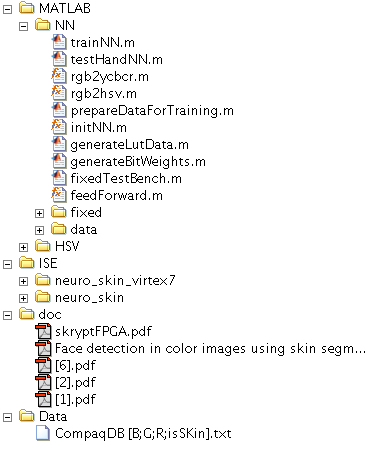
\includegraphics[width=0.63\linewidth]{images/tree.png}
\caption{Struktura katalogów}
\label{fig:tree}
\end{figure}

\begin{itemize}
\item \textbf{MATLAB} - folder zawierający wszystkie utworzone pliki środowiska MATLAB.
\begin{itemize}
\item \textbf{NN}
\begin{itemize}
\item \textit{trainNN.m} - skrypt trenujący model sieci neuronowej.
\item \textit{testHandNN.m} - skrypt testujący sieć na przykładowym obrazie.
\item \textit{generateLutData.m} - skrypt generujący dane dla LUTa w module języka verilog.
\item \textit{generateBitWeights.m} - skrypt generujący linijki kodu veriloga odpowiadające za przechowywanie wartości wag sieci neuronowych.
\item \textit{fixedTestBench.m} - test bench dla skryptów feedForward oraz fix\_feedforward.
\item \textit{feedForward.m} - funkcja symulująca moduł neural\_networks.v na liczbach zmiennoprzecinkowych
\item \textit{fix\_feedForward.m} - funkcja symulująca moduł neura\_networks.v na liczbach stałoprzecinkowych
\item data - folder zawierający zapisane modele sieci Neuronowych (wagi) oraz testowe obrazy.
\end{itemize}
\item \textbf{HSV} - folder zawierający skrypty wykorzystane do testowania modułu rgb2hsv zaimplementowanego w veriolgu.
\end{itemize}
\item \textbf{ISE} - folder zawierający projekty realizowane w środowisku ISE.
\begin{itemize}
\item \textit{neuro\_skin} - projekt finalny realizowany na kartę Spartan-6.
\item \textit{neuro\_skin\_virtex7} - projekt finalny przerzucony na tor wizyjny karty virtex7 (z projektu pbas)
\end{itemize}
\item \textbf{doc} - folder zawierający wykorzystane artykuły naukowe. Artykuł dostarczony przez prowadzącego jest opisany pełnym tytułem, pozostałe są oznaczone odnosząc się do jego bibliografii.
\item \textbf{Data} - folder zawierający bazę danych wykorzystaną do trenowania sieci neuronowej. (Compaq Database - \url{https://archive.ics.uci.edu/ml/machine-learning-databases/00229/Skin_NonSkin.txt})
\end{itemize}